%%%%%%%%%%%%%%%%%%%%%%%%%%%%%%
%% Paquetes
%%%%%%%%%%%%%%%%%%%%%%%%%%%%%%

\documentclass[conference]{IEEEtran}
\usepackage{blindtext, graphicx}
\usepackage[backend=biber]{biblatex}
\usepackage[spanish,mexico]{babel}
\usepackage[utf8]{inputenc}
\usepackage{csquotes}
\usepackage{amsmath}
\usepackage{amsfonts}
\let\labelindent\relax
\usepackage{enumitem}
\usepackage{paralist}
\usepackage[table]{xcolor}% http://ctan.org/pkg/xcolor
\usepackage{array}
\newcolumntype{L}[1]{>{\raggedright\let\newline\\\arraybackslash\hspace{0pt}}m{#1}}
\newcolumntype{C}[1]{>{\centering\let\newline\\\arraybackslash\hspace{0pt}}m{#1}}
\newcolumntype{R}[1]{>{\raggedleft\let\newline\\\arraybackslash\hspace{0pt}}m{#1}}
\definecolor{intnull}{RGB}{213,229,255}



\def\Var{{\rm{Var}}}
\def\E{{\rm{E}}}
\def\VarN{{\rm{Var_N}}}
\def\EN{{\rm{E_N}}}
\def\VarR{{\rm{Var_R}}}
\def\ER{{\rm{E_R}}}
\def\bsq#1{\lq{#1}\rq} %both single quotes
\def\ni{\noindent}
\def\RA{\Rightarrow}
\def\imps{\quad \RA \quad }
\def\bimps{\RA \quad }
\def\bqed{\quad_{\blacksquare}}

\addbibresource{bibliography.bib} %Imports bibliography file

%%%%%%%%%%%%%%%%%%%%%%%%%%%%%%
%% Funciones definidas
%%%%%%%%%%%%%%%%%%%%%%%%%%%%%%

\newcommand{\norm}[1]{\left\lVert#1\right\rVert}
 

% correct bad hyphenation here
\hyphenation{op-tical net-works semi-conduc-tor}


\begin{document}
% paper title
% can use linebreaks \\ within to get better formatting as desired
\title{Generación de listas de reproducción a través de comunidades de artistas en un grafo}


% author names and affiliations
% use a multiple column layout for up to three different
% affiliations
\author{\IEEEauthorblockN{Tania Mendoza Smith}
\IEEEauthorblockA{ITAM \\
Email: taniamendozas@gmail.com}
\and
\IEEEauthorblockN{Mario Becerra}
\IEEEauthorblockA{ITAM \\
Email: mario.becerra@itam.mx}
\and
\IEEEauthorblockN{Miguel Vilchis}
\IEEEauthorblockA{ITAM\\
Email: mvilchis@ciencias.unam.mx}}

% make the title area
\maketitle


\begin{abstract}
El objetivo de este trabajo es generar una lista de reproducción
a partir de artistas similares. Se usa un conjunto de datos que contine las canciones reproducidas por usuarios en un tiempo determinado. Transformamos los datos en un grafo para poder aplicar algoritmos de  detección de comunidades, y así obtener grupos de cada género. 
\end{abstract}

\section{Introducción}

El estudio de redes ha sido de gran interés en los últimos años. Estas permiten representar un conjunto de actores y las relaciones entre ellos de una manera intuitiva y con una representación visual. Muchos sistemas pueden ser modelados por medio de redes. Por ejemplo, relaciones entre páginas de internet, redes de transporte, redes de parentescos y redes sociales como \textit{Facebook} o \textit{Twitter}. Las redes comúnmente son modeladas por medio de grafos, ya sea direccionales o no direccionales. 

El análisis de los grafos generados a partir de distintas redes puede ser utilizado para encontrar características de los datos subyacentes de las redes. Ejemplos de esto son: encontrar las páginas web más importantes sobre algún tema; definir comunidades en un grafo social como \textit{Facebook} o \textit{Twitter}, o incluso en una red telefónica; o calcular el camino más corto de un punto a otro en una red de transporte.

Este trabajo se centra en un uso menos común del modelo de red: una red de artistas musicales generada a partir de la similutud entre ellos usando filtrado colaborativo sobre el histórico de reproducciones de \textit{LastFM}. El objetivo final será encontrar comunidades sobre esta red para generar \textit{estaciones de radio} a partir de comunidades de artistas similares.

\section{Metodología}

Para lograr el objetivo de este trabajo, se necesitan solucionar dos problemas distintos. Por un lado, se necesita generar una red de artistas a partir del histórico de reproducciones. Para esto, se hace un cálculo de similitud entre cada pareja de artistas para colocar arcos entre aquellos que tengan una similitud alta. Posteriormente, se quieren encontrar comunidades en esta red para generar una lista de reproducción.

Existen diversas metodologías para resolver ambos problemas, y se detallarán a continuación tanto la metodología elegida como algunas alternativas.

\section{Cálculo de la similitud}

Dado un conjunto de $n$ productos, un grupo de $m$ usuarios y una asignación de calificaciones de los usuarios a un subconjunto de los productos, se puede generar una matriz de calificaciones $R$ de dimensión $m \times n$ . Ejemplos de los productos pueden ser objetos que se venden en un sitio de \textit{e-commerce}, o películas, canciones y videos en un servicio de \textit{streaming}. Cada renglón la matriz $R$ contiene las calificaciones que asignó el usuario a cada producto. En la mayoría de los problemas, el usuario no califica explícitamente los productos, sino que se tienen calificaciones implícitas, inferidas a partir del comportamiento del usuario. Por ejemplo, valores binarios que indican una compra, o conteos de reproducción en \textit{Netflix}, \textit{YouTube} o \textit{Spotify}.

Un ejemplo de la matriz $R$ es el siguiente:

\begin{center}
    \begin{tabular}{ c | c  c c c c}
        & $C_1$ & $C_2$ & $C_3$ & $\cdots$ & $C_n$ \\
      \hline                       
      $U_1$ &   1 &     2 &     3 & $\cdots$ &      0 \\
      $U_2$ &   4 &     0 &     4 & $\cdots$  &     0\\
      $\vdots$ & $\vdots$ & $\vdots$ & $\vdots$ & $\ddots$ & $\vdots$\\
      $U_m$ &   0 &     0 &     1 & $\cdots$ &      3\\
      \hline  
    \end{tabular}
\end{center}


donde $C_i$ es el $i$-ésimo producto y $U_i$ es el $i$-ésimo usuario. Si la matriz estuviera representando reproducciones de canciones de usuarios, la entrada $(i, j)$ representaría el número de veces que el usuario $i$ escuchó la canción $j$. Es usual que este tipo de matrices tengan la mayor parte de las entradas igual a $0$, pues casi siempre hay una gran cantidad de productos a ofrecer, y los usuarios no pueden escuchar tantas canciones, ver tantos videos, o comprar tantos productos.

Si se quisiera calcular una medida de similitud entre cada pareja de productos, se podrían construir vectores a partir de las columnas de la matriz $R$, los cuales representan vectores de usuarios, de tal forma que para cada canción $i$ se tenga un vector $x_i \in \mathbb{R}^m$, donde la $k$-ésima entrada del vector $x_i$ sea el número de veces que el usuario $k$ escuchó la canción $i$, i.e., $x_i$ es la $i$-ésima columna de la matriz $R$. Después de tener estos vectores, se puede calcular una medida de similitud, como por ejemplo, la similitud coseno, la cual está definida para dos vectores $x, y \in \mathbb{R}^k$:

\begin{equation}
\label{eq:cosine_sim}
    \mathrm{sim}(x, y) = \frac{x^T y}{\norm{x} \norm{y}} = \frac{\sum_{i = 1}^k x_i y_i}{\sqrt{\sum_{i = 1}^k x_i^2}\sqrt{\sum_{i = 1}^k y_i^2}}.
\end{equation}

Como usualmente en este tipo de problemas se tienen una gran cantidad de productos y usuarios, al calcular las similitudes a partir de los vectores columna de $R$ uno se enfrenta a la maldición de la dimensionalidad (\textit{curse of dimensionality}), pues $m$ es grande. Este problema hace que las medidas de similitud no sean de utilidad, ya que se vuelven muy pequeñas siempre, haciendo difícil distinguir entre productos cercanos y lejanos  \cite{beyer1999nearest}.

\subsection{Mínimos Cuadrados Alternados}

Para evitar el problema anterior, es deseable reducir la dimensionalidad. Una de las maneras para reducirla es mediante la factorización de la matriz de calificaciones $R$. Como se mencionó anteriormente, tener un \textit{feedback} implícito es diferente a tener uno explícito. En este trabajo, se tiene un \textit{feedback} implícito en el comportamiento, por lo que se utiliza un método que toma en cuenta esta particularidad, y el cual está explicado en \cite{hu2008collaborative}. 

La finalidad del algoritmo de factorización es descomponer a la matriz $R$ en dos matrices de rango bajo de tal forma que el producto de estas se aproxime a la matriz original. Es decir, se busca encontrar dos matrices $U$ y $C$, con $U \in \mathbb{R}^{m \times f}$ y $C \in \mathbb{R}^{n \times f}$, con $f \ll \mathrm{min}(m, n)$, tales que $R \approx UC^T$.

Se define una función que mide el nivel de confianza de que $r_{ui} > 0$ de la siguiente forma

\[
    \gamma_{ui} = 1 + \alpha r_{ui}
\]

con $\alpha > 0$. Esta función nos permite tratar los feedbacks implícitos como ratings.

La $f$ es el número deseado de \textbf{factores latentes} de $R$. De esta forma, la calificación de un usuario $u$ a un producto $p$ es una combinación lineal de estos factores latentes.

\[
    R_{ij} = \sum_{k = 1}^f U_{ik} C_{jk}
\]

donde $U_{ik}$ es la entrada $(i, k)$ de $U$ y $C_{jk}$ es la entrada $(j, k)$ de $C$.

Ahora, la similitud entre productos se puede calcular a partir de la matriz $C$ donde cada renglón representa a cada producto en términos de sus factores latentes. Esta matriz tiene una dimensión considerablemente menor a la matriz original $R$, por lo que evitamos el problema de dimensionalidad.

El algoritmo que utilizamos para encontrar estas matrices de rango bajo se llama \textit{Alternate Least Squares}, es decir, mínimos cuadrados alternados. Se utiliza la función objetivo dada por la ecuación (\ref{eq:loss_func}).

\begin{equation}
    \label{eq:loss_func}
    \min_{u, c} \sum_{(j, k)} \gamma_{jk} \left( p_{j, k} - u_j^T c_k \right)^2 + \lambda \left( \sum_j \norm{u_j}^2 + \sum_k \norm{c_k}^2 \right) 
\end{equation}

La minimización por mínimos cuadrados alternados es un proceso iterativo en el cual se inicia con una matriz aleatoria $C$ y se obtiene $U$ a partir de optimizar (\ref{eq:loss_func}), posteriormente se fija $U$ y se optimiza (\ref{eq:loss_func}) para obtener $C$.

En cada iteración, se resuelve un problema de optimización en un tiempo de orden $O(p^2N + p^3 (m + n))$, donde $N$ es el número total usuarios que consumieron al menos un producto. Si el número máximo de iteraciones es $l$, entonces el obtener la matriz $C$ tiene una complejidad de orden $O(l (p^2N + p^3 (m + n)))$.



\section{Detección de Comunidades}

 
El objetivo final de este proyecto es identificar comunidades en un grafo en el que los nodos representan artistas musicales, y las aristas representan similitud entre ellos, para a partir de estas formar grupos de artistas a partir de los cuáles se puede generar una lista de reproducción.

Existen distintos tipos de algoritmos para detección de comunidades, algunos son divisivos, en el sentido que detectan ligas inter-comunidad y después los quitan de la red; otros son aglomerativos, ya que van juntando nodos recursivamente; y otros están basados en la maximización de una función objetivo.

Cabe mencionar, que el problema de detección de comunidades es radicalmente distinto al problema de particionar los vértices de un grafo. Esta diferencia fundamental yace en que el problema de partición tiene dado de antemano el número de grupos que se desea obtener, o el tamaño de éstos, es decir, existe información a priori de lo que se busca. Por otro lado, el problema de detección de comunidades tiene como objetivo encontrar la \textit{estructura subyacente} que agrupa a los nodos de un grafo sin información a priori sobre cómo es esta estructura de grupos. Se podría decir que el problema de detección de comunidades busca encontrar la partición natural de estos nodos.

Para nuestro problema, decidimos utilizar un algoritmo basado en la maximización de una función objetivo. Esta función objetivo es la modularidad, que será explicada a continuación. 




\subsection{Modularidad}

La modularidad es una de las medidas más populares para detectar comunidades en redes. Parte de esta popularidad se debe a que se han desarrollado algoritmos muy rápidos para maximizarla. También a que esta medida, a diferencia de otras, no se centra en características locales de la red, sino que ve la estructura global. La modularidad está en el intervalo $(-1,1)$ y busca medir la estructura de comunidad de una red.

Gracias a que la definición de comunidad es muy abierta, cada medida puede darle su propia interpretación y buscar características distintas en la separación. En el caso de la modularidad, se prefieren grupos con conexiones fuertes entre los miembros y débiles entre nodos de distintas comunidades. De manera más formal, se busca que existan menos aristas entre nodos de distintas comunidades de las \textit{esperadas}. Las aristas esperadas se calculan con un modelo nulo, la elección de este modelo cambia los resultados. El modelo normalmente utilizado es el modelo nulo de Newman-Girvan, ya que respeta la distribución de grados de la red. Este es el modelo nulo que se utilizará en este trabajo.

La modularidad $Q$ se calcula como la proporción de arcos que están dentro de cada comunidad menos el número esperado de arcos en cada comunidad de un grafo aleatorio con la misma distribución de grados (modelo nulo Newman-Girvan). Esto nos da la siguiente ecuación \cite{blondel_fast_2008}

\[
    Q = \frac{1}{2m} \sum_{i,j} (A_{ij} - \frac{k_i k_j}{2m}) \delta (c_i, c_j),
\]

donde $A_{ij}$ representa el peso del arco entre los nodos $i$ y $j$; $k_i = \sum_j A_{ij}$ es la suma de los pesos de los arcos que salen del nodo $i$; $c_i$ es la comunidad que se le asigna al vértice $i$; $\delta(u,v)$ es $1$ si $u=v$ y $0$ en otro caso; y $m = \frac{1}{2} \sum_{ij} A_{ij}$ es peso total de los arcos de la red.

Una limitante de utilizar la modularidad como función objetivo, es que puede fallar en encontrar comunidades pequeñas en una red muy grande. Esto se debe a que se resta el número esperado de vértices, el cual va disminuyendo conforme la red crece, volviéndo un término despreciable y provocando que la medida junte dos grupos pequeños en una misma comunidad. Esta limitante puede ser una ventaja en nuestra aplicación particular, pues balanceará el tamaño de las comunidades.

\subsection{Algoritmo de Louvain}

Encontrar la partición óptima de acuerdo a la modularidad es un problema NP, ya que implicaría explorar todas los posibles agrupamientos y elegir el que maximice la medida. Por ello, existen algoritmos que exploran solo una parte del espacio de soluciones. 

Para optimizar la modularidad, haremos uso del algoritmo de Louvain \cite{Blondel08fastunfolding}. Este algoritmo fue creado en el 2007 y es uno de los más rápidos. Es un algoritmo \textit{greedy} que en cada iteración busca mejorar el valor de la modularidad. 

El algoritmo se divide en varias corridas, cada una consistente de 2 fases. En cada iteración de fases, se hará uso del cálculo de la \textit{ganancia en modularidad}. La ganancia está dada por la siguiente fórmula:

\begin{align}
\begin{split}
    \Delta Q = \left[  \frac{ \sum_{C} +  d_{i,C} }{  2m  }  - \left( \frac{ \sum_{adj} +  d_{i} }{2m} \right)^2  \right] - \\
    \left[ \frac{ \sum_{C} }{2m}  -  \left( \frac{\sum_{adj} }{ 2m } \right)^2 - \left( \frac{ d_i }{ 2m } \right)^2 \right],
\end{split}
\end{align}

donde

$ \sum_{C} = \sum_{j,k \in C} w_{jk}$,

$ d_{i,C} = \sum_{j \in C} w_{ij}$, y

$  \sum_{adj} = \sum_{j\in C k \notin C} w_{jk}$.
 
\bigskip
El proceso se inicia con una gráfica $G$ con $n$ nodos.
\begin{compactenum}
\item[] \textbf{Fase 1:}
\item Asignarle a cada nodo su propia comunidad, es decir, en principio tenemos $n$ comunidades.
\item Para cada nodo $v_{i}$, nos fijamos en sus $d_{i}$ vecinos y evaluamos la \textit{ganancia en modularidad} que resultaría de quitar a $v_{i}$ de su propia comunidad y ponerlo en la de cada uno de sus vecinos. 
\item Ponemos a $v_{i}$ en la comunidad del vecino $v_{j}$ que dé la mayor ganancia, siempre y cuando esta sea estrictamente positiva. En caso de no existir movimiento que suponga una ganancia positiva, dejamos a $v_{i}$ en su propia comunidad.
\item Este proceso se repite secuencialmente para todos los nodos hasta que no se pueda obtener mejoría de hacer estos movimientos individuales. En esta fase se obtiene un óptimo local.
\end{compactenum}
\medskip 


\begin{compactenum}
\item[] \textbf{Fase 2:}
\item Construimos una nueva gráfica donde las comunidades encontradas en la fase 1 se vuelven nodos. 
\item Ahora, las aristas tendrán pesos, que se construyen sumando los pesos de las aristas entre comunidades, de la siguiente manera:

    $$\hat{w_{ij}} = \sum_{v_{k} \in C_{i}, v_{l} \in C_{k}} w_{kl} ,$$

donde $\hat{w_{ij}}$ es el peso de los nodos formados por la comunidad $i$ y la comunidad $j$ y $w_{kl}$ es el peso de la arista entre el nodo $v_k$ y $v_l$ si esta arista existe. Las aristas entre nodos de una misma comunidad se vuelven lazos. Cabe mencionar que si iniciamos con una gráfica sin pesos, tomamos $w_{kl}=1$ para toda arista $v_kv_l\in E$.
\end{compactenum}
\medskip

El algoritmo sigue corriendo hasta que no se encuentre mejoría en la modularidad, y en cada corrida el número de comunidades, claramente, va decreciendo. 

La razón por la que el método resulta tan rápido es por lo fácil que es calcular la ganancia en modularidad al hacer un cambio. 

\subsection{Limitantes de la Modularidad y el Algoritmo de Louvain}

Existen algunas limitantes al usar la modularidad como medida de detección de comunidades, así como de usar el algoritmo de Louvain. Por un lado, la medida de modularidad tiene un \textit{límite de resolución}. Esto se refiere a que la modularidad puede ser incapaz de identificar comunidades naturales, dando particiones muy gruesas, es decir, sobreagrupando. Este límite depende del tamaño total de la gráfica y de qué tan conectados estén sus nodos. Podemos encontrar dos casos peligrosos en los que la partición se vería afectada por este límite:
\begin{compactenum}
    \item Dos comunidades tienen un balance perfecto entre aristas dentro de la comunidad y aristas fuera de él. Así que están en el límite de conformar una comunidad.
    \item Dos comunidades tienen una única arista conectándolas con el resto de la gráfica, y sólo una arista conectándolas al uno con el otro. En este caso, el método de modularidad no podría separarlas aunque se tratara de dos gráficas completas unidas por una única arista.
\end{compactenum}

En nuestra aplicación, este comportamiento de hecho puede resultar beneficioso, pues los grupos de artistas tendrán aproximadamente el mismo tamaño, lo que se traduce en listas de reproducción con tamaños similares.


Así mismo, es importante notar que por la naturaleza aleatoria del inicio del algoritmo, la partición resultante depende del orden en el que se revisan los nodos. Para mejorar este problema, en la práctica, se corren varios procesos completos con inicios aleatorio y se toma el que da el mejor resultado. Los autores del algoritmo de Louvain indican que este algoritmo podría resolver el problema de resolución de la modularidad, usando las soluciones intermedias como soluciones alternativas, aunque esto no ha probado ser cierto \cite{Fortunato201075}.


%\subsection{\textit{Centralidad de Intermediación}}
%
%La \textit{centralidad de intermediación} mide el número de veces que un nodo actúa como puente en el camino más corto entre dos nodos. Es una forma de cuantificar el control que tiene  un nodo en la comunicación existente entre otros. La idea básica detrás de esta medida es que los nodos con mayor \textit{centralidad} son los que aparecen con mayor probabilidad en los caminos más cortos, de esta forma, es una medida de centralidad en una red. Esta medida está dada por la siguiente ecuación \cite{sun_survey_2011},
%
%\begin{equation}
%C_{BET}(i)=\sum_{j,k}\frac{b_{jik}}{b_{jk}} 
%\end{equation}
%
%donde $b_{jk}$ es el número de caminos más cortos desde el nodo j hasta el nodo $k$, y $b_{jik}$ el número de caminos más cortos desde $j$ hasta $k$ que pasan a través del nodo $i$.
%
%Los nodos con un alto valor de intermediación son muy importantes en la estructura de una red, ya que comunican comunidades con otras. Comúnmente los valores más altos de \textit{betweenness} son obtenidos por los nodos que están en los bordes de las comunidades. Si uno nodo con alta intermediación desaparece, las comunidades podrían quedar incomunicadas. Calcular el \textit{betweenness} resulta ser una tarea complicada y tardada, pues se recorre toda la red nodo por nodo, por esto han surgido métodos que intentan optimizarlo, como el algoritmo de intermediación de Girvan-Newman.
%
%Esta noción de centralidad en los nodos se puede extender a las aristas, y de esta forma el \textit{betweenness} de una arista es el número de caminos más cortos entre el par de nodos que corren a través de esta arista. Así, las aristas que conectan comunidades tendrán mayor nivel de \textit{betweenness}, pues al quitar estas aristas, las comunidades quedarían separadas una de la otra. Esta noción de \textit{betweenness} de aristas se puede explotar para encontrar comunidades en la red. El algoritmo Girvan-Newman hace esto siguiendo los siguientes pasos:
%
%\begin{enumerate}
%\item Se calcula el \textit{betweenness} de cada arco
%\item Se quita el arco con mayor \textit{betweenness}
%\item Se recalcula el \textit{betweenness} de los arcos afectados por la acción de haber quitado el arco
%\item Se repiten los pasos 2 y 3 hasta que no queden más arcos
%\end{enumerate}
%
%Este algoritmo devuelve un dendrograma en el cual las hojas son los nodos, con esto se pueden asignar comunidades a los nodos.
%



\section{Implementación}

Nuestro objetivo es generar listas de reproducción a partir de artistas similares. Una opción para decidir que dos artistas son similares podría ser a partir de características explícitas de su música, por ejemplo, usando el género. Sin embargo, decidimos que sería mejor tomar información de los gustos de las personas a partir de su comportamiento de reproducción. Contamos con la información de reproducción de al rededor de mil usuarios en \textit{LastFM}.
Una vez calculada la similitud entre artistas, queremos agruparlos para generar listas de reproducción. Para esto, generamos una red y usamos el algoritmo de detección de comunidades para partirla en grupos.

\subsection{Obtención de información y preprocesamiento}

La información de reproducción fue tomada de \textit{LastFM}. El dataset contiene el id de usuario, id de canción, nombre de canción, id de artista, nombre de artista y un timestamp de la fecha y hora de reproducción. Decidimos trabajar usando el id del usuario y el id de artista de la lista de reproducción. De esta manera, podemos generar una matriz de reproducción, donde a cada usuario le corresponde un vector de artistas y las entradas están dadas por el número de veces que escuchó alguna canción de ese artista.
\begin{center}
     \begin{tabular}{ c | c  c c c c}
         & $A_1$ & $A_2$ & $A_3$ & $\cdots$ & $A_n$ \\
       \hline                       
       $U_1$ &   1 &     2 &     3 & $\cdots$ &      0 \\
       $U_2$ &   4 &     0 &     4 & $\cdots$  &     0\\
       $\vdots$ & $\vdots$ & $\vdots$ & $\vdots$ & $\ddots$ & $\vdots$\\
       $U_m$ &   0 &     0 &     1 & $\cdots$ &      3\\
      \hline  
   \end{tabular}
\end{center}

En esta matriz, $A_i$ es el $i$-ésimo artista y $U_i$ es el $i$-ésimo usuario. Así, la entrada $(i, j)$ representa el número de veces que el usuario $i$ escuchó una canción del artista $j$. Es usual que este tipo de matrices tengan la mayor parte de las entradas igual a $0$, pues no todos los usuarios han escuchado todas las canciones.

Como parte de la preparación de los datos, nos deshicimos de aquellos usuarios que hubieran escuchado \textit{pocas} canciones, ya que no proveen información. La decisión de corte fue hecha a partir de un histograma, y decidimos eliminar a los usuarios que hubieran escuchado menos de 10 artistas distintos. Bajo un razonamiento similar, nos deshicimos de aquellos artistas que solo hubieran sido reproducidos por una misma persona.

\subsection{Similitud entre artistas}

Primero se define la matriz binaria de reproducciones $R$ tal que la entrada $(u, i)$, denotada por $r_{ui}$, es tal que 

\[   
r_{ui} = 
     \begin{cases}
       1 \text{ si } R_{ui} > 0 \\
       0 \text{ si } R_{ui} = 0, \
     \end{cases}
\]

donde $R_{ui}$ es el número de veces que el usuario $i$ escuchó al artista $i$. Si $R_{ui} > 0$ hay indicio de que al usuario $u$ le gusta el artista $i$, si $R_{ui} = 0$ no hay tal indicio. Sin embargo, los indicios pueden tener distintos niveles de confianza pues, debido a la naturaleza de los datos, el hecho de que $R_{ui} = 0$ se puede deber a distintos factores, como que el usuario no conoce tal artista, o que no está disponible, o que en efecto, no es de su agrado. Así mismo, el hecho de que $R_{ui} > 0$ puede ser debido a que el usuario escuchó esa canción porque era la que seguía de otra canción que sí le gusta al usuario. En general, mientras más grande sea $R_{ui}$, hay más indicio de que a $u$ le gusta $i$.

Una forma de calcular la similitud entre cada par de artistas podría ser construyendo vectores de usuarios, como se mencionó anteriormente, de tal forma que para cada artista $i$ se tenga un vector $x_i \in \mathbb{R}^m$, donde la $k$-ésima entrada del vector $x_i$ sea el número de veces que el usuario $k$ escuchó una canción del artista $i$, pero debido a la maldición de la dimensionalidad, usamos filtrado colaborativo para encontrar factores latentes en el espacio de los artistas utilizando la descomposición de matrices, de tal forma que se encuentran dos matrices $U$ y $A$ tales que su producto aproxime a $R$.

Las matrices $U$ y $A$ se pueden interpretar en función de los factores latentes. La matriz $U$ representaría a los usuarios en términos de sus gustos y la matriz $A$ a los artistas en términos de sus características latentes. Cada fila de $U$ es un usuario, y el valor de cada entrada $k$ de la fila explica qué tan inclinado está hacia el factor $k$; y análogamente, cada fila de $A$ es un artista, y cada entrada $k$ explica qué tan inclinado está el artista hacia el factor $k$, con $k \in \left\{1, \cdots, p \right\}$.

Para el cálculo de la matriz $A$, utilizamos la técnica descrita en la sección anterior de mínimos cuadrados alternados. Usamos 10 iteraciones y decidimos generar una matriz de rango 20, es decir, $f = 20$. De esta manera, cada artista tendrá un vector con 20 entradas que representan el valor que toma en cada uno de los factores latentes. Cabe mencionar, que algunos de estos factores podrían ser interpretados en términos de qué representan haciendo un análisis sobre los valores. Se podría determinar, por ejemplo, que el factor 1 corresponde a \textit{qué tan} pop es una canción, o \textit{qué tan} rápida o lenta es. Sin embargo, un análisis de este tipo no resulta pertinente a nuestro objetivo.

Una vez que se tiene la matriz $A$, se calculan todos los pares de similitudes de artistas usando la similitud coseno en la ecuación \ref{eq:cosine_sim}. Esta es una operación con una complejidad de orden $O(n^2)$, por lo que puede ser tardado calcularla. Si el tiempo de ejecución fuera algo crucial, se podría utilizar una heurística como vecinos más cercanos aproximados (\textit{approximate nearset neighbors}), en la cual, para los $k$ vecinos más cercanos que se quieran calcular, el tiempo de ejecución es de orden $O(kn \log{n})$ \cite{arya1994optimal}.

\subsection{Matriz de artistas por similitud}

Una vez que obtuvimos la similitud para todas las parejas de artistas, podemos formar la red. El primer paso para esto fue filtrar las similitudes que consideramos no relevantes, ya que no queríamos una red completamente conectada, sino una red con estructura de comunidad, es decir, con conexiones solo entre nodos relevantes. Filtramos con dos criterios:

\begin{compactenum}
    \item Eliminamos todas las similitudes negativas. Esto porque en nuestro problema, el vector de factores representa características y una diferencia de signo para alguna de estas características implica lejanía. Estas diferencias de signo son capturadas como un valor negativo de la similitud coseno.
    \item Eliminamos todas las similitudes menores a $0.4$. El valor fue elegido haciendo uso una vez más de un histograma. Consideramos que valores menores de similitud meterían ruido en la topología de nuestra red.
\end{compactenum}

La red de similitudes se puede expresar como una matriz de adyacencias $S$ donde para la pareja de artistas $(i,j)$ existe una arista solo si su similitud es mayor o igual a $0.4$. La entrada $S_{ij} = sim_{ij}$, es decir que peso del arco está dado por el valor de la similitud. 

A partir de esta red, corrimos el algoritmo de detección de comunidades para encontrar un agrupamiento \textit{natural} de los artistas que resultan similares y que por lo tanto resultan buenos candidatos para formar una lista de reproducción, por ejemplo.

También se utilizó la api de \textit{Spotify} para comparar los resultados obtenidos, eso se hizo a través de la libreria \textit{Rspotify} para el lenguaje \textit{R}. 

\section{Resultados}

Después de aplicar la metogología al conjunto de datos descrito obtuvimos 14 comunidades (o \textit{clusters}), donde cada uno representa un género. El número de artistas por cada comunidad se puede ver en la Tabla I y en la Figura 1. Se puede ver los artistas que más representan a cada comunidad, en el sentido de que son los que mayor número de reproducciones tienen, en las Tablas II y III.

\begin{table}[ht]
\centering
\label{table:numero_artistas_comunidad}
\caption{Número de artistas en cada comunidad}
\begin{tabular}{|c|c|}
  \hline
 Comunidad & Número de artistas \\ 
  \hline
1 & 3297 \\ 
2 & 3872 \\ 
3 & 3555 \\ 
4 & 5920 \\ 
5 & 2425 \\ 
6 & 3880 \\ 
7 & 7905 \\ 
8 & 4677 \\ 
9 & 2135 \\ 
10 & 3461 \\ 
11 & 5711 \\ 
12 & 6408 \\ 
13 & 3348 \\ 
14 & 2263 \\ 
   \hline
\end{tabular}
\end{table}

\begin{figure}[h]
    \centering
    \label{fig:numero_artistas_comunidad}
    \caption{Número de artistas en cada comunidad}
    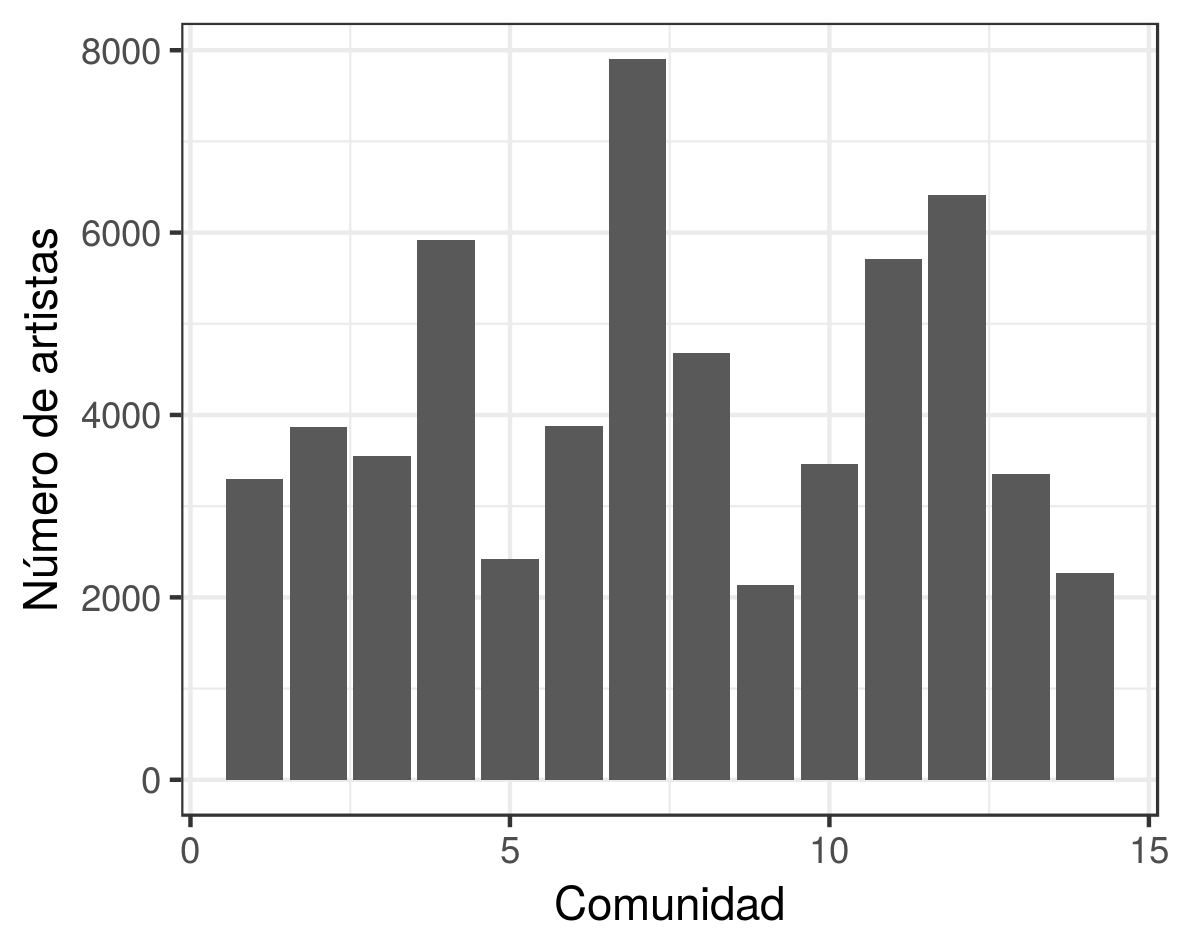
\includegraphics[width=5cm]{artistas_por_comunidad.png}
\end{figure}
\begin{table}[]
\label{table:artistas_representantes_comunidad}
\caption{Artistas con mayor número de reproducciones en cada comunidad}
\centering
\begin{tabular}{|c|c|}
  \hline
 Comunidad & Artista \\ 
  \hline
1 & The String Quartet \\ 
1 & The Black Angels \\ 
1 & Tunng \\ 
1 & The Warlocks \\ 
1 & Can \\ 
1 & Nits \\ 
1 & Black Mountain \\ 
1 & Hawkwind \\ 
1 & The Brian Jonestown Massacre \\ 
1 & Rachel'S \\ \hline
2 & Dispatch \\ 
2 & Ozric Tentacles \\ 
2 & Elio E Le Storie Tese \\ 
2 & Biosphere \\ 
2 & Eluvium \\ 
2 & Easy Star All-Stars \\ 
2 & Stars Of The Lid \\ 
2 & Shpongle \\ 
2 & Coil \\ 
2 & King Crimson \\   \hline
3 & Myslovitz \\ 
3 & Apparat \\ 
3 & Mando Diao \\ 
3 & Max Richter \\ 
3 & Seeed \\ 
3 & Venetian Snares \\ 
3 & Ellen Allien \& Apparat \\ 
3 & Die Fantastischen Vier \\ 
3 & Kult \\ 
3 & Burial \\  \hline
4 & Sloan \\ 
4 & Bel Canto \\ 
4 & De-Phazz \\ 
4 & Gotan Project \\ 
4 & Bonobo \\ 
4 & Nightmares On Wax \\ 
4 & The Radio Dept. \\ 
4 & Red House Painters \\ 
4 & The Cinematic Orchestra \\ 
4 & Rocky Votolato \\  \hline
5 & Nujabes \\ 
5 & Build An Ark \\ 
5 & Pop Levi \\ 
5 & Dabrye \\ 
5 & Jamie Lidell \\ 
5 & Over The Rhine \\ 
5 & Cut Chemist \\ 
5 & Flying Lotus \\ 
5 & Ammoncontact \\ 
5 & Madlib \\  \hline
6 & Aesop Rock \\ 
6 & Crystal Castles \\ 
6 & Justice \\ 
6 & Kent \\ 
6 & Wu-Tang Clan \\ 
6 & Mew \\ 
6 & T.I. \\ 
6 & Eminem \\ 
6 & Rjd2 \\ 
6 & Kanye West \\  \hline
7 & Gwen Stefani \\ 
7 & Soda Stereo \\ 
7 & Britney Spears \\ 
7 & Shakira \\ 
7 & Rihanna \\ 
7 & Skinny Puppy \\ 
7 & Christina Aguilera \\ 
7 & Justin Timberlake \\ 
7 & P!Nk \\ 
7 & Mindless Self Indulgence \\ \hline
\end{tabular}
\end{table}


\begin{table}[]
\label{table:artistas_representantes_comunidad_pt2}
\caption{Artistas con mayor número de reproducciones en cada comunidad (Parte 2)}
\centering
\begin{tabular}{|c|c|}
  \hline
 Comunidad & Artista \\ 
  \hline
8 & Windy \& Carl \\ 
8 & Flight Of The Conchords \\ 
8 & Blue Man Group \\ 
8 & Butthole Surfers \\ 
8 & Meat Puppets \\ 
8 & Lightning Bolt \\ 
8 & Townes Van Zandt \\ 
8 & Faust \\ 
8 & The Legendary Pink Dots \\ 
8 & The Residents \\  \hline
9 & Pegboy \\ 
9 & Jme \\ 
9 & Vivian Girls \\ 
9 & Nashville Pussy \\ 
9 & Roky Erickson \\ 
9 & Smoking Popes \\ 
9 & Milton Nascimento \\ 
9 & The Evens \\ 
9 & The Georgia Satellites \\ 
9 & The Gutter Twins \\  \hline
10 & Engenheiros Do Hawaii \\ 
10 & Indochine \\ 
10 & Humanwine \\ 
10 & Buena Vista Social Club \\ 
10 & John Coltrane \\ 
10 & Madeleine Peyroux \\ 
10 & Riverside \\ 
10 & Herbie Hancock \\ 
10 & Chet Baker \\ 
10 & Django Reinhardt \\  \hline
11 & Linkin Park \\ 
11 & Evanescence \\ 
11 & A Perfect Circle \\ 
11 & In Flames \\ 
11 & The 69 Eyes \\ 
11 & Porcupine Tree \\ 
11 & Children Of Bodom \\ 
11 & Soilwork \\ 
11 & Afi \\ 
11 & Nightwish \\  \hline
12 & Nine Inch Nails \\ 
12 & Pink Floyd \\ 
12 & Elliott Smith \\ 
12 & Depeche Mode \\ 
12 & The Beatles \\ 
12 & Radiohead \\ 
12 & Coldplay \\ 
12 & Placebo \\ 
12 & Muse \\ 
12 & Death Cab For Cutie \\  \hline
13 & Lyfe Jennings \\ 
13 & Nellie Mckay \\ 
13 & Deus \\ 
13 & Secret Machines \\ 
13 & Youth Group \\ 
13 & Afterhours \\ 
13 & Lucero \\ 
13 & Annuals \\ 
13 & The Stills \\ 
13 & The Frames \\  \hline
14 & Uverworld \\ 
14 & High And Mighty Color \\ 
14 & Soundtrack \\ 
14 & M-Flo \\ 
14 & L'Arc\~{}En\~{}Ciel \\ 
14 & Dir En Grey \\ 
14 & T.M.Revolution \\ 
14 & Acidman \\ 
14 & Bonnie Pink \\ 
14 & Chemistry \\ 

   \hline
\end{tabular}
\end{table}
\newpage
Para conocer la calidad de la división, tomamos como representante del grupo a los artistas con mayor número de reproducciones. Seguido de eso, usamos la API de \textit{Spotify}, para encontrar los artistas relacionados con cada representante.


La lista que obtenemos del API de \textit{Spotify} contiene 20 artistas relacionados, seguido de esto,  
buscamos a cada uno de los artistas en el grupo del representante. Se espera que los 20 artistas 
se encuentren en la comunidad del representante.

En promedio, los artistas relacionados que se encontraron en el mismo grupo que el artista representante fueron $40.3 \%$. Con los siguientes resultados: 


\begin{tabular}{|L{2.5cm}|C{2.5cm} |C{2.5cm} |}
\label{tab:artistas_encontrados_count}
 \hline
& Número de grupos & Artistas encontrados de 20\\ \hline
Mejores casos & 3 & 18 \\ \hline
Peores casos & 3 & 0 \\ \hline
Caso promedio & 8 & 7.9 \\ \hline
\end{tabular}


El grupo $12$ representa uno de los  mejores grupos, ya que, de los $20$ artistas relacionados con el representante del grupo, $18$ se encontraron dentro de nuestro grupo. 
Los artistas con mayor número de reproducciones del grupo se muestran
en la siguiente tabla: 

\begin{tabular}{|L{3.5cm}|L{3.5cm} |}
\label{tab:relaciones}
\multicolumn{2}{c}{Grupo 12}\\ \hline
     \textbf{Artistas  con más reproducciones} & \textbf{Artistas relacionados con Radiohead (Spotify)} \\ \hline
               Radiohead   & \cellcolor{intnull}  Radiohead \\ \hline
           The Beatles	   & \cellcolor{intnull}     Blur        \\ \hline
       Nine Inch Nails	   & \cellcolor{intnull}  The Flaming Lips \\ \hline       
                  Muse	   & \cellcolor{intnull}  Arcade Fire    \\ \hline
              Coldplay	   & \cellcolor{intnull}  Pixies        \\ \hline
          Depeche Mode	   & \cellcolor{intnull}  Interpol       \\ \hline 
            Pink Floyd	   & \cellcolor{intnull}  Portishead      \\ \hline  
   Death Cab For Cutie	   & \cellcolor{intnull}  Beck        \\ \hline
               Placebo	   & \cellcolor{intnull}  Sonic Youth    \\ \hline    
         Elliott Smith	   & \cellcolor{intnull}  Wilco        \\ \hline
              The Cure	   &          PJ Harvey        \\ \hline
           David Bowie	   &\cellcolor{intnull}   The Smashing Pumpkins \\ \hline
           The Killers	   &\cellcolor{intnull}   My Bloody Valentine    \\ \hline
            The Smiths	   &    LCD Soundsystem        \\ \hline
 Red Hot Chili Peppers	   &\cellcolor{intnull}   Sigur Rós     \\ \hline   
             Metallica	   &\cellcolor{intnull}   Joy Division   \\ \hline     
              Interpol	   &\cellcolor{intnull}   Animal Collective \\ \hline       
            Bloc Party	   & \cellcolor{intnull}  Grizzly Bear   \\ \hline     
 Black Rebel Motorcycle Club &	\cellcolor{intnull} Pulp       \\ \hline 
           Arcade Fire	     & \cellcolor{intnull}  Placebo      \\ \hline  
 Modest Mouse	             & \cellcolor{intnull}  Björk   \\ \hline 
\end{tabular}

Del lado izquierdo se muestran los artistas con mayor número de reproducciones del grupo, mientras que del lado izquierdo los artistas relacionados con el representante del grupo, es decir  los artistas relacionados con $Radiohead$, obtenidos de la API de \textit{Spotify}. Además, se sombrearon los artistas relacionados que se encuentran en el grupo. 

El peor caso lo representan el grupo 2, 3 y 14, ya que en estos no se encontró ningun artista relacionado con el representante dentro del grupo.

Para conocer qué género representa cada grupo, nos apoyamos en la API de \textit{Spotify}, tomando todos los artistas pertenecientes a cada 
grupo y por cada uno de ellos se obtuvo el género. La distribución de los géneros por cada grupo se puede ver en la Figura 2. 

\begin{figure}[h]
    \centering
    \label{fig:dist_generos}
    \caption{Distribución de los géneros en cada comunidad}
    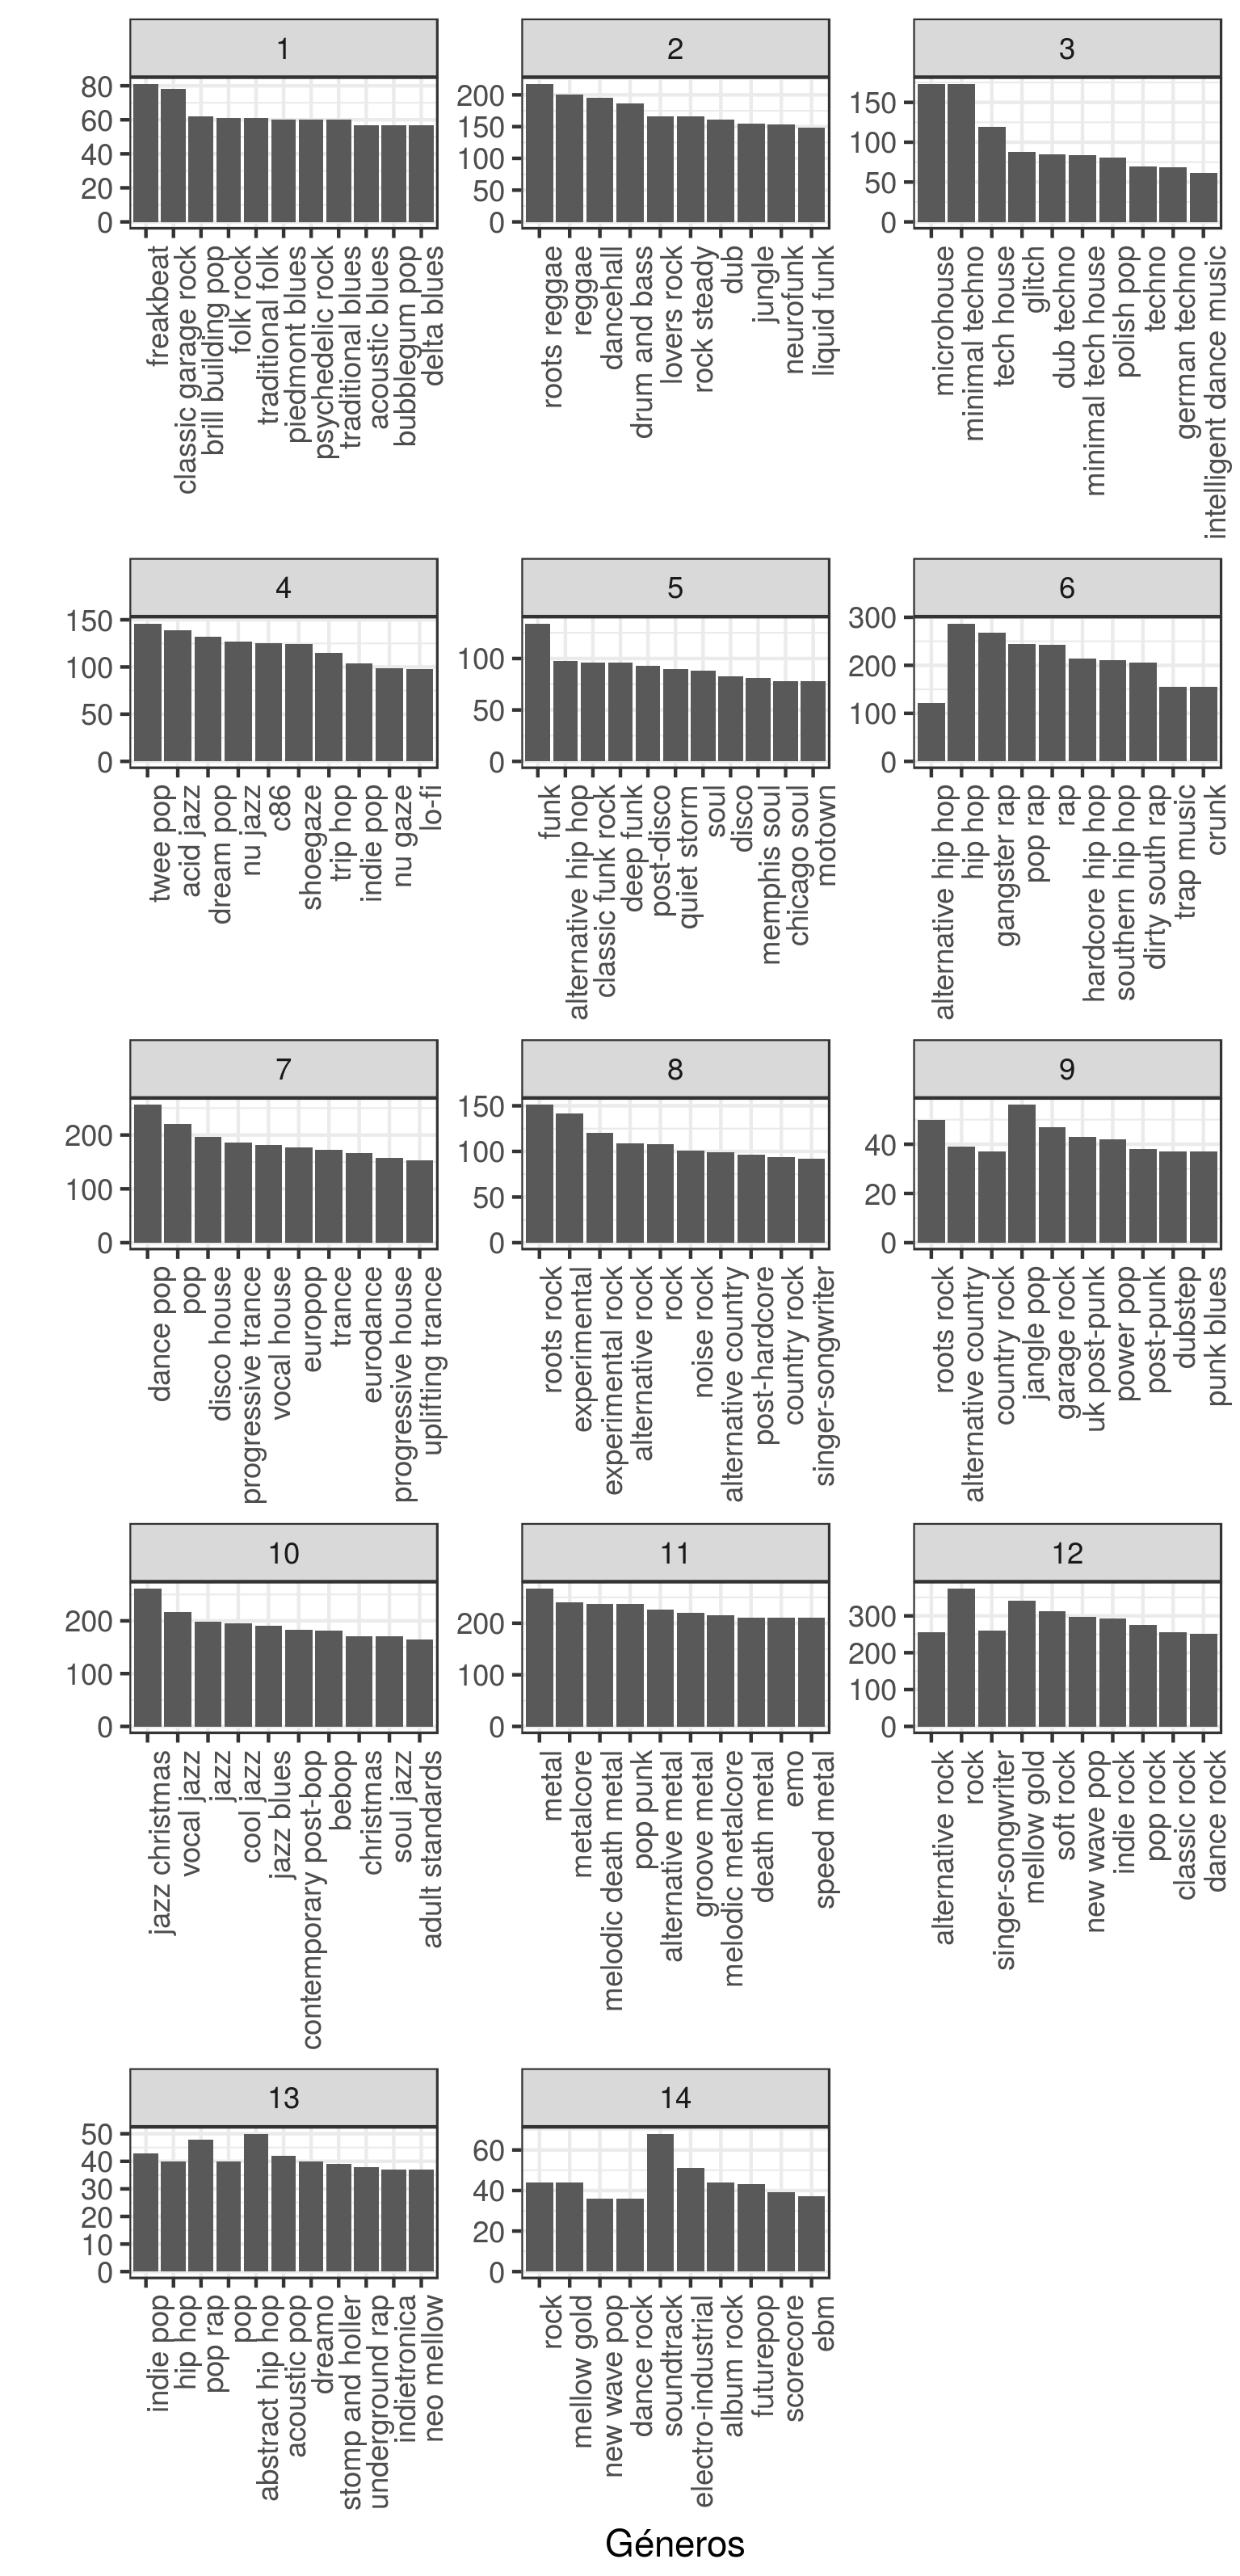
\includegraphics[width=8.5cm]{generos_plot_2.png}
\end{figure}

\printbibliography
\nocite{*}




\end{document}